\documentclass{book}
\usepackage{hyperref}
\usepackage{graphicx}


\title{Documentazione}
\author{Benedetta Vitale - Emilio Meroni}
\date{\today}


\begin{document}

\maketitle

\tableofcontents    

\chapter{Project Plane}

\begin{figure}[ht]
        \centering
        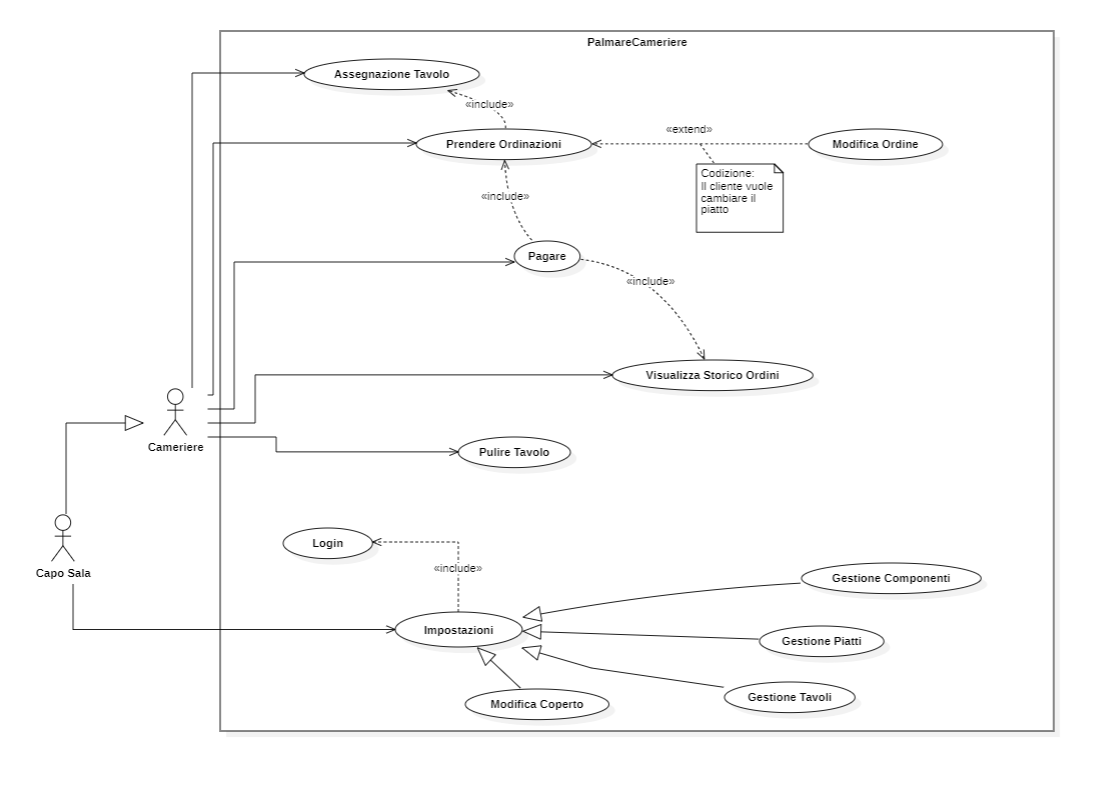
\includegraphics[width=1\linewidth]{../../UML/Diagrammi/Use_Case_Diagram.png}
        \caption{Use Case Diagram}
        \label{fig: use_case_diagram}
      \end{figure}

\section{Introduzione}


Questo progetto verrà svolto da Benedetta Vitale ed Emilio Meroni, 
entrambi studenti al terzo anno di ingegneria informatica presso 
l'università di Bergamo.

Il software che andremo a sviluppare è pensato per dare supporto 
alla attività di ristorazione. In particolare, dovrà assistere alle mansioni dei camerieri, come ad esempio prendere le ordinazioni ai tavoli, redigere il conto, trovare tavoli disponibili, ecc.

Abbiamo scelto questa tipologia di sistema dato che Emilio lavora, nei week-end, presso un ristorante, e gli ha incuriosito la gestione interna tramite l'utilizzo dei palmari da parte dei camerieri. 

\section{Modello di Processo}

Il modello di processo che abbiamo deciso di seguire e quello della prototipazione, in particolare la prototipazione evolutiva, molto utile per quanto riguarda la costruzione dell'interfaccia grafica, la parte principale della nostra applicazione

\section{Organizzazione del Progetto}

Utilizzeremo una organizzazione a tre livelli:

\begin{enumerate}
    \item Livello Data Base
    \item Livello Logico
    \item Livello Presentazione
\end{enumerate}

Il \textit{livello Data Base}, come da nome, si occuperà della parte del DB, il quale sarà embedded, SQLite.
Il \textit{livello Presentazione} sarà quello visto dall'utente che usufruirà dell'applicazione, possiamo definirlo come il livello più esterno dove i dati verranno presentati in modo grafico e la gestione dei tavoli e delle comande è fatto in modo interattivo.
L'ultimo livello è quello \textit{Logico}, il quale possiamo posizionarlo graficamente tra il livello Data Base e quello Presentazione, funge da intermediario tra i due livelli e fornisce gli oggetti principali per la gestione dell'applicazione


\section{Standard, Lineeguida, Procedure}

Come standard abbiamo scelto di utilizzare lo standard definita da \textit{Java} , il quale si può trovare su questo

\section{Attività di Gestione}

\section{Rischi}

\section{Personale}

\section{Metodi e Tecniche}

\section{Garanzia e Qualità}

Il programma dovrà essere utilizzato in ristoranti, e in particolare dal personale che prenderà le ordinazioni, quindi dovrà essere di \textit{facile} utilizzo, con un focus maggiore sulla funzionalità che sull'estetica. Un'altra qualità che dovrà garantire è la \textit{prevenzione di errori} da parte degli utenti, come ad esempio il "miss-click" (click errati o accidentali).
In particolare abbiamo evidenziato quattro qualità che sistema dovrà possedere, di cui, per ciascuna indichiamo come garantiremo che verrà seguito:

\begin{enumerate}
    \item \textbf{Semplice}: programma sara scritto per avere poche sezioni scritte e di facile comprensione, anche per chi si approcia al programma per la prima volta. Si utilizzeranno poche schermate che contengono tutto il necessario per le \textit{macro} operazioni definite nelle specifiche dei requisiti e indicate nel case diagram [Figura: \ref{fig: use_case_diagram}].
    \item \textbf{Intuiblile}: Utilizzo dei colori per indicare gli stati dei \textit{tavoli}, in particolre si è deciso che per i \textit{tavoli liberi} su utilizzara il colore verde, per i \textit{tavoli occupati} il colore rosso e per i \textit{tavoli da pulire} l'arancione
    \begin{figure}[h]
        \centering
        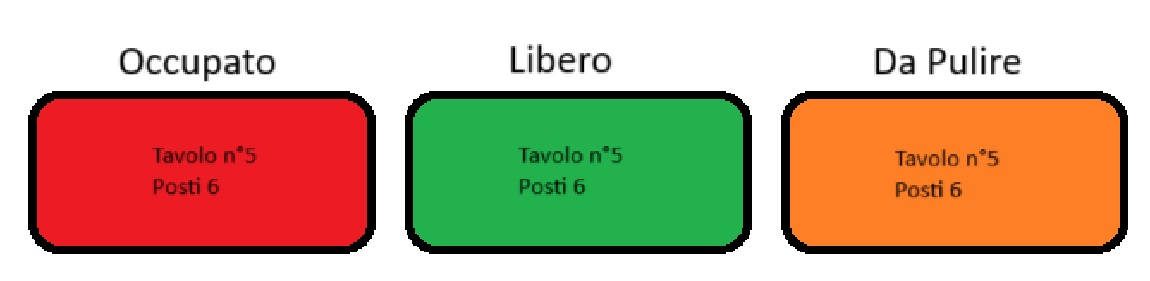
\includegraphics[width=0.6\linewidth]{../../Immagini/Esempio_Bottoni.jpg}
        \caption{Esempio Bottoni}
        \label{fig: es_bottoni}
    \end{figure}
    \item \textbf{Prevenzione Errori}: feedback visivo
    \item \textbf{Veloce}:
\end{enumerate}

È semplice e intuibile perché ha poche scritte di facile comprensione, anche per chi si approccia al programma per la prima volta al programma; ci sono poche schermate che hanno al loro interno tutto il necessario per le operazioni che si desiderano; inoltre, i bottoni e i colori rendono il programma semplice e intuibile. È veloce in quanto il programma ha poche sezioni in cui bisogna utilizzare la testiera, mentre il programma è più focalizzato sull'uso dei bottoni che lo rendono molto più veloce nelle azioni che si dovranno svolgere. Il programma è Prevenzione Errori dato che, con le schermate pop-up di conferma, c'è una riduzione dei possibili errori che si possono creare nell'uso del programma.


\section{Workpackages}

\section{Risorse}

\section{Budget}

\section{Cambiamenti}

% futuro sistema di log-in

\section{Consegna}

In questa sezione si discutono i metodi e le scadenze di consegna del progetto, in particolare la consegna si dividerà in due fasi:


\begin{itemize}
    \item Consegna del \textit{Project Plane}, il quale dovrà essere consegnato circa un mese prima del primo esame scritto, che si svolgerà nel mese di gennaio; quindi, per il mese di dicembre si dovrà effettuare la prima consegna.
    \item Consegna del \textit{Progetto}, quest'ultimo avrà una scadenza più lunga, infatti, l'ultimo giorno di consegna sarà cinque giorni prima dell'esame orale.
\end{itemize}
Per quanto riguarda i metodi di consegna si dovrà condividere con il professore Gargantini la repository di github contenente il progetto, per la consegna di questo documento si dovrà indicare nel file reame, della repository, la posizione del project plane. Mentre per la consegna del progetto si dovrà creare un issue, intitolata “Approvazione Progetto” ed assegnarla al professore.



\end{document}